\documentclass{article}

\title{Learning Incoherent Subspaces: Classification via Incoherent Dictionary Learning.}

\author{Daniele Barchiesi and Mark D. Plumbley}
%\affiliation{Centre for Digital Music\\
%	Queen Mary University of London\\
%	Mile End Road, London E1 4NS, UK}

%%%%%%%%%%%%%%%%%%%%%%PACKAGES%%%%%%%%%%%%%%%%%%%%%
\usepackage{amsmath,graphicx}
\usepackage[english]{babel}
\usepackage[applemac]{inputenc}
\usepackage[T1]{fontenc}
\usepackage{epsfig}
\usepackage{amsfonts,amssymb,amsmath,amsthm,bm}
\usepackage[boxruled,linesnumbered]{algorithm2e}
\usepackage{subfig,graphicx}
\usepackage{setspace}
\usepackage{enumitem}

%%%%%%%%%%%%%%%%%%%%%DEFINITIONS%%%%%%%%%%%%%%%%%%
/Users/daniele/Dropbox/Career/Research/MyPapers/Projects/2013-MLSP/definitions.tex	


\def \nComponents{L} 	%number of significant components of ICA feature transform
\def \fea{\Vector{x}} 	%vector of features
\def \Feas{\Matrix{X}} 	%matrix containing set of training features
\def \iFea{n}	 		%component index of features vector
\def \nDim{N} 			%dimensionality of features vector
\def \newFea{\Vector{y}} 	%features vector after feature transform
\def \NewFeas{\Matrix{Y}}%matrix of training features after feature transform
\def \Dic{\Matrix{\Phi}} %dictionary learned from features
\def \nAto{K} 			%number of atoms in the dictionary
\def \iAto{k} 			%atom index
\def \atom{\Vector{\phi}}%atom in a dictionary
\def \nFea{M}			%number of signals or features
\def \iFea{m}			%signal index
\def \Coeff{\Matrix{A}} 	%matrix of sparse approximation coefficients
\def \coherence{\mu} 		%mutual coherence
\def \coeff{\Vector{\alpha}}%vector of sparse approximation coefficients
\def \nActiveAtoms{S} 	%number of active atoms
\def \orthmat{\Matrix{W}} 	%orthonormal matrix
\def \cat{c} 			%category
\def \cats{\Vector{c}}	%vector of categories of training signals
\def \Cat{\mathcal{C}} 	%set of possible categories
\def \uniCat{C} 			%element of the set of possible categories
\def \iCat{p}  		%index of the elements in the set of possible categories
\def \nCat{P} 		%number of elements in the set of possible categories
\def \definition{\overset{\Label{def}}{=}}	%definitions
\def \Gram{\Matrix{G}} 						%Gram matrix
\def \gram{g} 								%element of the Gram matrix
\def \admissibleDictionary{\Function{D}} 	%set of admissible dictionaries
\def \ambient{\Set{R}} 						%ambient
\def \ipr{\Acronym{ipr}} 					%Iterative projections and rotations
\def \ip{\Acronym{ip}}						%Iterative projections
\def \nDimSub{Q}
\def \Spa{\Matrix{\Psi}}

\begin{document}
%\ninept
%

\maketitle
%
\begin{abstract}

\end{abstract}
%
%\begin{keywords}
%Feature transforms, sparse approximation, dictionary learning, supervised classification.
%\end{keywords}
%
\section{Introduction: Classification And Feature Transforms}\label{sec:intro}
Supervised classification is one of the classic problems in machine learning where a system is designed to discriminate the category of an observed signal, having previously observed representative examples from the considered classes \cite{Duda1973Pa}.

Typically, a classification algorithm consists of a training phase where  class-specific models are learned from labelled samples, followed by a testing phase where unlabelled data are classified by comparison with the learned models. Both training and testing comprise various stages. Firstly, we observe a signal that measures a process of interest, such as the recording of a sound or image, or a log of the temperatures in a particular geographic area. Then, a set of features are extracted from the raw signals using signal processing techniques. This step is performed in order to reduce the dimensionality of the data and provide a new signal that allows generalisation among examples of the same class, while retaining enough information to discriminate between different classes. 

Following the features extraction step, a feature transform can be employed to further reduce the dimensionality of the data and to enhance discrimination between classes. Thus classification benefits from feature transforms especially when features are not separable, that is, when it is not possible to optimise a simple function that maps features belonging to signals of a given class to the corresponding category. 
A further dimensionalty reduction may be performed when dealing with high dimensional signals (such as audio or high resolution images) by fitting the parameters of global statistical distributions with features learned on portions of the signal. Models learned on different classes are finally compared using a distance metric to the model learned form an unlabelled signal, which is typically assigned to the nearest class.

\subsection{Traditional Algorithms For Feature Transform}\label{sec:aft}
Two of the main feature transform techniques include principal component analysis (\Acronym{pca}) \cite{Pearson1901On} and Fisher's linear discriminant analysis (\Acronym{lda}) \cite{Duda1973Pa}.

\subsubsection{\Acronym{pca}}

Let $\curlyb{\fea_{\iFea} \in \real^{\nDim}}_{\iFea=1}^{\nFea}$ be a set of vectors containing features extracted from $\nFea$ training signals. The goal of \Acronym{pca} is to learn an orthonormal set of basis functions $\curlyb{\atom_{\iAto} \in \ambient^{\nDim}}_{\iAto=1}^{\nDim}$ such that $ \norm{\atom_{\iAtom}}{2}=1$ and $\inner{\atom_{i}}{\atom_{j}}=0 \; \forall i\neq j$ that are placed along the columns of a so-called \emph{dictionary} $\Dic\in\real^{\nDim\times\nDim}$. The bases are optimised from the data to identify their principal components, that is, the sub-spaces that retain the maximum variance of the features.

To compute the dictionary, the eigenvalue decomposition of the outer product
\begin{equation}
\Matrix{X}\Transpose{\Matrix{X}} = \Matrix{Q}\Matrix{\Lambda}\Transpose{\Matrix{Q}}
\end{equation}
is first calculated. Then, the $\nComponents$ eigenvectors corresponding to the $\nComponents$ largest eigenvalues are selected from the matrix $\Matrix{Q}$, and scaled to unit $\ell_{2}$ norm to form the dictionary $\Dic$.

Let $\Spa\definition\Dic_{1:\nComponents}\in\ambient^{\nDim\times\nComponents}$ denote the sub-dictionary constructed from the $\nComponents<\nDim$ principal components of the dataset. A new set of transformed features $\newFea_{\Acronym{pca}} = \Spa\Transpose{\Spa}\fea$ is computed by projecting the data onto the sub-space spanned by the columns of $\Dic_{1:\nComponents}$ (that is, onto the $\nComponents$-dimensional principal sub-space). This operation reduces the dimensionality of the features by projecting them onto a linear subspace embedded in $\real^{\nDim}$. It is an unsupervised technique that does not exploit knowledge about the classes associated with the training set, but implicitly relies in the assumption that the principal component directions encode relevant differences between classes.

\subsubsection{\Acronym{lda}}
In contrast, \Acronym{lda} is a supervised method for feature transform whose objective is to explicitly maximise the separability of classes in the transformed domain. 

Let $\obsSet_{\iUniCat}$ be a set indexing features extracted from data belonging to the $\iUniCat$-th category, let
\begin{equation}
\average{\fea}_{\iUniCat} \definition \frac{1}{\abs{\obsSet_{\iUniCat}}}\sum_{\iObs\in\obsSet_{\iUniCat}} \fea_{\iObs}
\end{equation} 
be the $\iUniCat$-th class feature centroid, and $\average{\fea}\definition\sum_{\iObs=1}^{\nObs}\fea_{\iObs}$ the centroid of the features extracted from the entire training dataset. The between-classes scatter matrix 
\begin{equation}
\Matrix{S_{b}} \definition \sum_{\iUniCat=1}^{\nUniCat}\abs{\obsSet_{\iUniCat}}\roundb{\average{\fea}_{\iUniCat}-\average{\fea}}\Transpose{\roundb{\average{\fea}_{\iUniCat}-\average{\fea}}}
\end{equation} 
is defined to measure the mutual distances between the centroids of different classes, while the within-classes scatter matrix 
\begin{equation}
\Matrix{S}_{w}\definition \sum_{\iUniCat=1}^{\nUniCat}\sum_{\iObs\in\obsSet_{\iUniCat}}\roundb{\fea_{\iObs}-\average{\fea}_{\iUniCat}}\Transpose{\roundb{\fea_{\iObs}-\average{\fea}_{\iUniCat}}}
\end{equation}
quantifies the distances between features belonging to the same class.
To maximise an objective function $\objective(\Matrix{W})\definition\frac{\abs{\Transpose{\Matrix{W}}\Matrix{S}_{b}\Matrix{W}}}{\abs{\Transpose{\Matrix{W}}\Matrix{S}_{w}\Matrix{W}}}$ that promotes features belonging to the same class to be near each other and far away from features belonging to other classes, the eigenvalue decomposition of the matrix
\begin{equation}
\pseudoinverse{\Matrix{S}_{w}}\Matrix{S}_{b} = \Matrix{Q}\Matrix{\Lambda}\Transpose{\Matrix{Q}}
\end{equation}
is computed, and the features $\fea$ are projected onto the space spanned by its $(\nUniCat-1)$ eigenvectors corresponding to the largest $(\nUniCat-1)$ eigenvalues.

\Acronym{lda} explicitly seeks to enhance the discriminative power of features by optimising the objective $\objective$.
\subsection{Supervised dimensionality reduction}
\subsubsection{Supervised PCA}
Related works that extend \Acronym{pca} include the supervised \Acronym{pca} (\Acronym{s-pca}) proposed by Barshan et al. \cite{Barshan2011Su}. \Acronym{s-pca} is based on the theory of reproducing kernel Hilbert spaces (\Acronym{rkhs}) (that are spaces of functions which satisfy certain properties and map elements from an arbitrary set to the set of complex numbers) \cite{Aronszajn:1950}, and on the so-called Hilbert-Schmidt independence criterion (\Acronym{hsic})\cite{gretton2005measuring}. The \Acronym{hsic} is used to estimates the statistical dependence of two random variables based on the fact that this quantity is related to the correlation of functions belonging to their respective \Acronym{rkhs}. While \Acronym{hsic} is defined in terms of the probability density function of the two random variables,  empirical estimates of \Acronym{hsic} can be obtained from finite sequences of their realisations. The empirical \Acronym{hsic} can be used in turn to construct an objective function that maximises the dependence between the two variables. Hence, this strategy is adopted within the context of classification to maximise the statistical dependence between a transformed feature $\newFea_{\Acronym{s-pca}}$ and its corresponding category $\cat$.

In practice, \Acronym{s-pca} differs from \Acronym{pca} in that it calculates the eigenvalue decomposition of a matrix $\Matrix{R}$ defined as follows:
\begin{equation}
\Matrix{R} \definition \Matrix{X}\Matrix{H}\Matrix{L}\Matrix{H}\Transpose{\Matrix{X}}
\end{equation}
were $\Matrix{H} \definition \Matrix{I} - \Vector{e}\Transpose{\Vector{e}}$ is a \emph{centring} matrix and $\Matrix{L} \definition \Vector{\cat}\Transpose{\Vector{\cat}}$ is the kernel matrix of the class variable that is constructed by computing the outer product of the vectors resulting from assigning different numerical values to each category. 

Other methods for supervised dimensionality reduction include metric learning algorithms \cite{xing2002distance}, sufficient dimensionality reduction \cite{li1991sliced} and supervised principal components \cite{Bair06predictionby}.

\subsection{Incoherent subspace learning and other related work}


and methods for manifold learning reviewed by Van Der Maaten et al. \cite{Van-Der-Maaten2009Di}. Finally, the sparse sub-space clustering technique developed by Elhamifar and Vidal \cite{Elhamifar2013Sp} applies concepts and algorithm from the field of sparse approximation to tackle unsupervised clustering problems.


\subsection{Main Contributions and Paper organisation}
The method proposed in this paper is aimed at learning discriminative sub-spaces that allow dimensionality reduction, while at the same time enhancing the separability between classes. It is derived from our previous work on learning incoherent dictionaries for sparse approximation.

Standard methods for feature transform will be briefly reviewed in Section \ref{sec:aft}, as their limitations lead to the main motivation for this work. To provide the context of the proposed method, the incoherent dictionary learning problem will be introduced in Section \ref{sec:idl}, while Section \ref{sec:lis} will contain the main contribution of this paper consisting in learning incoherent subspaces for classification. Numerical experiments are presented in Section \ref{sec:ne}, and conclusions are drawn in Section \ref{sec:end}.

\section{Incoherent Dictionary Learning}\label{sec:idl}
A sparse approximation of a signal $\fea\in\real^{\nDim}$ is a linear combination of $\nAto\geq\nDim$ basis functions $\curlyb{\atom_{\iAto}\in\real^{\nDim}}_{\iAto=1}^{\nAto}$ called \emph{atoms} described by:
\begin{equation}
	\fea \approx \approximant{\fea} = \sum_{\iAto=1}^{\nAto} \alpha_{\iAto}\atom_{\iAto}
\end{equation}
where the vector of coefficients $\coeff$ contains a \emph{small} number of non-zero components, corresponding to a small number of atoms actively contributing to the approximation $\approximant{\fea}$. Given a signal $\fea$ and a dictionary, various algorithms have been proposed to find a sparse approximation that minimises the residual error $\norm{\fea-\approximant{\fea}}{2}$\cite{Elad2010Sp}.

Dictionary learning aims at optimising a dictionary $\Dic$ for sparse approximation given a set of training data. It is an unsupervised technique that can be thought as being a generalisation of \Acronym{pca}, as both methods learn linear subspaces that minimise the approximation error of the signals. Dictionary learning, however, is generally more flexible than \Acronym{pca} because it can be employed to learn more general non-orthogonal over-complete dictionaries \cite{Rubinstein2010Di}.

\subsection{The incoherent dictionary learning problem}
Dictionaries for sparse approximation have important intrinsic properties that describe the relations between their atoms, like the mutual coherence $\mu(\Dic)=\underset{i\neq j}{\max}{\inner{\atom_{i}}{\atom_{j}}}$ that is defined as the maximum inner product between any two different atoms. The goal of incoherent dictionary learning is to learn atoms that are well adapted to sparsely approximate a set of training signals, and that are at the same time mutually incoherent \cite{Barchiesi2013Le}. 

Given a set of $\nFea$ training signals contained in the columns of the matrix $\Feas \in \real^{\nDim\times\nFea}$ and a matrix $\Coeff\in\real^{\nAto\times\nFea}$ indicating the sparse approximation coefficients, the incoherent dictionary learning problem can be expressed as:

\begin{align}\label{eq:iprcost}
\optimal{\Dic} = \MinimiseST{\Dic}{\norm{\Feas-\Dic\Coeff}{\F}}{\coherence(\Dic) \leq \coherence_{0} \nonumber \\
			&\norm{\coeff_{\iFea}}{0}\leq \nActiveAtoms \quad \forall \iFea}
\end{align}
where $\coherence_{0}$ is a fixed mutual coherence constraint, the $\ell_{0}$ pseudo-norm $\norm{\cdot}{0}$ counts the number of non-zero components of its argument and $\nActiveAtoms$ is a fixed number of active atoms. Algorithms for (incoherent) dictionary learning generally follow an alternate optimisation heuristic, iteratively updating $\Dic$ and $\Coeff$ until a stopping criterion is met. In the case of the iterative projections and rotations algorithm (\Acronym{ipr}) algorithm \cite{Barchiesi2013Le}, a dictionary de-correlation step is added after updating the dictionary in order to satisfy the mutual coherence constraint. 

Given $\Feas$, fixed $\coherence_{0}$, $\nActiveAtoms$ and a stopping criterion (such as a maximum number of iterations), the optimisation of \eqref{eq:iprcost} is tackled by iteratively performing the following steps:
\begin{itemize}
	\item\emph{Sparse coding}: fix $\Dic$ and compute the matrix $\Coeff$ using a suitable sparse approximation method.
	\item\emph{Dictionary update}: fix $\Coeff$ and update $\Dic$ using a suitable method for dictionary learning.
	\item\emph{Dictionary de-correlation}: given $\Feas$, $\Dic$ and $\Coeff$ update the dictionary $\Dic$ to reduce its mutual coherence under the level $\coherence_{0}$.
\end{itemize}

\subsection{The iterative projections and rotations algorithm}\label{sec:ipr}
The \Acronym{ipr} algorithm has been proposed in order to solve the dictionary de-correlation step, while ensuring that the updated dictionary provides a sparse approximation with low residual norm, as indicated by the objective function \eqref{eq:iprcost} \cite{Barchiesi2013Le}.

The \Acronym{ipr} algorithm requires the calculation of the Gram matrix $\Gram=\Transpose{\Dic}\Dic$ which contains the inner products between any two atoms in the dictionary. $\Gram$ is iteratively projected onto two constraint sets, namely the structural constraint set $\stcset$ and the spectral constraint set $\spcset$. The former is the set of symmetric square matrices with unit diagonal values and off-diagonal values with magnitude smaller or equal than $\coherence_{0}$:
\small
\begin{equation*}
	\stcset \definition \curlyb{\stcmat \in \ambient^{\nAtoms \times \nAtoms} : \stcmat = \Transpose{\stcmat}, \stcel_{i,i}=1,\max_{i > j}|\stcel_{i,j}|\leq \coherence_{0}}.
\end{equation*}
\normalsize
The latter is the set of symmetric positive semidefinite square matrices with rank smaller than or equal to $\nDimensions$:
\begin{equation*}
\spcset \definition \curlyb{ \spcmat \in \ambient^{\nAtoms \times \nAtoms} : \spcmat = \Transpose{\spcmat}, \operatorname{eig}(\spcmat)\geq \Vector{0}, \operatorname{rank}(\spcmat)\leq \nDimensions}
\end{equation*}  
where the operator $\operatorname{eig}(\cdot)$ returns the vector of eigenvalues of its argument.

Starting from the Gram matrix of an initial dictionary $\Dictionary$, the \Acronym{ipr} method iteratively performs the following operations.
\begin{itemize}
\item \emph{Projection onto the structural constraint set}. The projection $\stcmat = \Projection_{\stcset}(\Gram)$ can be obtained by:
\begin{enumerate}
\item setting $\stcel_{i,i} = 1$,
\item limiting the off-diagonal elements so that, for $i \neq j$, 
\small
\begin{equation}\label{eq:pscs}
\stcel_{i,j} = \operatorname{Limit}({\gram}_{i,j},\coherence_{0}) = \left\{ \begin{array}{rl}
	\gram_{i,j}  & \text{if} \quad |\gram_{i,j}|\leq \coherence_{0} \\
	\operatorname{sgn}(\gram_{i,j})\coherence_{0}  & \text{if} \quad |\gram_{i,j}| > \coherence_{0}
\end{array} \right.
\end{equation}
\normalsize
\end{enumerate}
\item \emph{Projection onto the spectral constraint set and factorization}. The projection $\spcmat = \Projection_{\spcset}(\Gram)$ and subsequent factorisation are obtained by:
\begin{enumerate}
\item calculating the eigenvalue decomposition (\Acronym{evd}) $\Gram = \eigvecmat \eigvalmat \Transpose{\eigvecmat}$,
\item thresholding the eigenvalues by keeping only the $\nDimensions$ largest positive ones.
\begin{equation*}
	\left[\operatorname{Thresh}(\eigvalmat,\nDimensions) \right]_{i,i} = \left\{ \begin{array}{rl}
	\lambda_{i,i}  & \text{if} \quad i \leq N \; \text{and} \; \lambda_{i,i}>0 \\
	0  & \text{if} \quad i > N \; \text{or} \; \lambda_{i,i}\leq 0
	\end{array}\right.
\end{equation*}
where the eigenvalues in $\eigvalmat$ are ordered from the largest to the smallest. Following this step, at most $\nDimensions$ eigenvalues of the Gram matrix are different from zero,
\item factorizing the projected Gram matrix into the product $\Gram=\Transpose{\Dic}\Dic$ by setting:
\begin{equation}
\Dic = \eigvalmat^{1/2}\Transpose{\eigvecmat}.
\end{equation}
\end{enumerate}
\item \emph{Dictionary rotation}. Rotate the dictionary $\Dic$ to align it to the training set by solving the problem:
\begin{equation}\label{eq:rot}
	\optimal{\orthmat} = \Minimise{\orthmat \Transpose{\orthmat} = \Matrix{I}}{\norm{\Feas - \orthmat\Dic\Coeff}{\Label{F}}}.
\end{equation}
The optimal rotation matrix can be calculated by:
\begin{enumerate}
\item computing the sample covariance between the observed signals and their approximations $\CovMat \definition (\Dic\Coeff)\Transpose{\Feas}$,
\item calculating the \Acronym{svd} of the covariance $\CovMat = \Matrix{U}\Matrix{\Sigma}\Transpose{\Matrix{V}}$,
\item setting the optimal rotation matrix to $\optimal{\orthmat}=\Matrix{V}\Transpose{\Matrix{U}}$,
\item rotating the dictionary $\Dic \leftarrow \optimal{\orthmat}\Dic$.
\end{enumerate}
\end{itemize}

More details about the \Acronym{ipr} algorithm can be found in  \cite{Barchiesi2013Le}, including details of its computational cost.
%The code of the \Acronym{ipr} method is illustrated in Algorithm \ref{algo:ipr}.
%
%\begin{algo}
%\KwIn{$\Feas, \Dictionary, \Coeff, \coherence_{0}, \nIter$}
%\KwOut{$\optimal{\Dictionary}$}
%$\iter\gets1$\;
%\While{$\iter \leq \nIter$ and $\coherence(\Dictionary)>\coherence_{0}$}{
%	\tcp{Calculate Gram matrix}
%	$\Gram \gets \Transpose{\Dictionary}\Dictionary$\;
%	\tcp{Project ont structural c.s.}
%	$\operatorname{diag(\Gram)} \gets \Vector{1}$\;
%	$\Gram \gets \operatorname{Limit}(\Gram,\coherence_{0})$\;
%	\tcp{Project Gram matrix onto spectral c.s. and factorize}
%	$[\eigvecmat, \eigvalmat] \gets \Acronym{evd}(\Gram)$\;
%	$\eigvalmat \gets \operatorname{Thresh}(\eigvalmat,\nDimensions)$\;
%	$\Dictionary \gets \eigvalmat^{1/2}\Transpose{\eigvecmat}$\;
%	\tcp{Rotate dictionary}
%	$\CovMat \gets \Feas\Transpose{(\Dictionary\Coeff)}$\;
%	$[\Matrix{U},\Matrix{\Sigma},\Matrix{V}] \gets \Acronym{svd}(\CovMat)$\label{algo:ipr:svd}\;
%	$\OrthMat \gets \Matrix{V}\Transpose{\Matrix{U}}$\;
%	$\Dictionary \gets \OrthMat\Dictionary$\;
%	$\iter\gets\iter+1$\;
%}
%\caption{\label{algo:ipr}Iterative projections and rotations (\Acronym{ipr})}
%\end{algo}


\section{Learning Incoherent Subspaces}\label{sec:lis}
The \Acronym{ipr} algorithm learns a dictionary where all the atoms are mutually incoherent. Therefore, given any two disjoint sets $\Lambda\bigcap\Gamma=\emptyset$ that identify non-overlapping collections of atoms, the sub-dictionaries $\Dic_{\Lambda}, \Dic_{\Gamma}$ are also mutually incoherent.

Starting from this observation, the main intuition driving the development of a supervised \Acronym{ipr} (\Acronym{s-ipr}) algorithm for classification is to learn mutually incoherent sub-dictionaries that approximate features from different classes of signals. The sub-dictionaries are in turn used to define incoherent sub-spaces, and features are projected onto these sub-spaces yielding discriminative dimensionality reduction. 
  
\subsection{The supervised \Acronym{ipr} algorithm}\label{sec:iprclass}
Let $\curlyb{\cat_{\iFea}\in\Cat}_{\iFea=1}^{\nFea},\; \Cat=\curlyb{\uniCat_{1},\uniCat_{2},\dots,\uniCat_{\nCat}}$ be a set of labels that identify the category of the vectors of features $\fea_{\iFea}$, whose elements belong to a set $\Cat$ of $\nCat$ possible categories. The columns of the matrix $\Feas_{\iCat}$ contain a selection of the features extracted from signals belonging to the $\iCat$-th category.

To learn incoherent sub-dictionaries from the entire set of features, we must first cluster the atoms to different classes\footnote{Note that the term \emph{cluster} implies that a this stage the algorithm needs to make an unsupervised decision, since there is no any a-priori reason to assign a given atom to any particular class.}, and then only proceed with their de-correlation  if they are assigned to different categories (while allowing coherent atoms to approximate features from the same class). To this aim, we employ the matrix $\Coeff$ to measure the contribution of every atom to the approximation of features belonging to each class.

Let $\coeff_{\iCat}^{\iAto}$ indicate the $\iAto$-th row of the matrix $\Coeff_{\iCat}$ containing the coefficients that contribute to the approximation of $\Feas_{\iCat}$, and $\nDim_{\iCat}$ indicate the number of its elements. A coefficient $\gamma_{\iAto,\iCat}$ is defined as:
\begin{equation}
	\gamma_{\iAto,\iCat} \definition \frac{1}{\nDim_{\iCat}}\norm{\coeff_{\iCat}^{\iAto}}{1},
\end{equation}
and every atom $\atom_{\iAtom}$ is associated with the category to which it maximally contributes $\optimal{\iCat}_{\iAto} = \underset{\iCat}{\arg\max}\curlyb{\gamma_{\iAto,\iCat}}$. 

Grouping together atoms that have been assigned to the same class leads to a set of sub-dictionaries whose size and rank depends on the number of atoms for each class, and to their linear dependence. As a general heuristic, if  features corresponding to different classes do not occupy the same sub-space (according to the active elements in $\Coeff$), a full-rank dictionary $\Dic$ with $\nAto \geq \nDim \gg \nCat$ ensures that $\optimal{\iCat}_{\iAto}$ identify $\nCat$ non-empty and disjoint sub-dictionaries $\curlyb{\Dic_{\iCat}}_{\iCat=1}^{\nCat}$.

Once the atoms have been clustered, the Gram matrix $\Gram$ is computed and iteratively projected as in the method described in Section \ref{sec:ipr}, with the difference that equation \eqref{eq:pscs} is modified in order to only constraint the mutual coherence between atoms assigned to different categories
\small
\begin{equation}\label{eq:pscs2}
\operatorname{Limit}({\gram}_{i,j},\coherence_{0},\optimal{\Vector{\iCat}}) = \left\{ \begin{array}{rl}
	\gram_{i,j}  & \text{if} \quad |\gram_{i,j}|\leq \coherence_{0} \, \text{or} \, \optimal{\iCat}_{i}=\optimal{\iCat}_{j} \\
	\operatorname{sgn}(\gram_{i,j}) \coherence_{0}  & \text{if} \quad |\gram_{i,j}|   >  \coherence_{0} \, \text{and} \, \optimal{\iCat}_{i}\neq\optimal{\iCat}_{j}
\end{array} \right.
\end{equation}
\normalsize


A further modification of the standard \Acronym{ipr} algorithm presented in \cite{Barchiesi2013Le} consists in the update of the Gram matrix, performed by computing its element-wise average with the projection $\stcmat = \Projection_{\stcset}(\Gram)$ (rather than by using the projection alone). This heuristic has led to improved empirical results by preventing $\Gram$ from changing too abruptly. 

The complete supervised \Acronym{s-ipr} method is summarised in Algorithm \ref{algo:sipr}. Note that the mutual coherence $\coherence_{\optimal{\iCat}}(\Dic) = \underset{\optimal{\iCat}_{i}\neq\optimal{\iCat}_{j}}{\arg\max}\inner{\atom_{i}}{\atom_{j}}$ indicated in this algorithm measures the inner product between any two atoms assigned to different categories since atoms assigned to the same category are allowed to be mutually coherent.
\begin{algo}
\KwIn{$\Feas, \Dictionary, \Coeff, \coherence_{0}, \cats, \nIter$}
\KwOut{$\optimal{\Dictionary}$}
$\iter\gets1$\;
\tcp{Cluster atoms}
$\Coeff_{\iCat} \gets \squareb{\coeff_{j}} \forall j \in \uniCat_{\iCat}$\;
$\gamma_{\iAto,\iCat} \gets \norm{\coeff_{\iCat}^{\iAto}}{1}/\nDim_{\iCat}$\;
$\optimal{\iCat}_{\iAto} = \underset{\iCat}{\arg\max}\curlyb{\gamma_{\iAto,\iCat}}$\;
\While{$\iter \leq \nIter$ and $\coherence_{\optimal{\iCat}}(\Dictionary)>\coherence_{0}$}{
	\tcp{Calculate Gram matrix}
	$\Gram \gets \Transpose{\Dictionary}\Dictionary$\;
	\tcp{Project onto structural c.s.}
	$\operatorname{diag}(\stcmat) \gets \Vector{1}$\;
	$\stcmat \gets \operatorname{Limit}(\Gram,\coherence_{0},\optimal{\Vector{\iCat}})$\;
	$\Gram \gets \frac{1}{2}\Gram + \frac{1}{2}\stcmat$\;
	\tcp{Project onto spectral c.s. and factorize}
	$[\eigvecmat, \eigvalmat] \gets \Acronym{evd}(\Gram)$\;
	$\eigvalmat \gets \operatorname{Thresh}(\eigvalmat,\nDimensions)$\;
	$\Dictionary \gets \eigvalmat^{1/2}\Transpose{\eigvecmat}$\;
	\tcp{Rotate dictionary}
	$\CovMat \gets \Feas\Transpose{(\Dictionary\Coeff)}$\;
	$[\Matrix{U},\Matrix{\Sigma},\Matrix{V}] \gets \Acronym{svd}(\CovMat)$\label{algo:ipr:svd}\;
	$\OrthMat \gets \Matrix{V}\Transpose{\Matrix{U}}$\;
	$\Dictionary \gets \OrthMat\Dictionary$\;
	$\iter\gets\iter+1$\;
}
\caption{\label{algo:sipr}Supervised \Acronym{ipr}}
\end{algo}
\subsection{Classification via incoherent subspaces}\label{sec:class}
The \Acronym{s-ipr} algorithm allows to learn a set of sub-dictionaries $\curlyb{\Dic_{\iCat}}$ that contain mutually incoherent atoms. These cannot be directly used to define discriminative subspaces because, depending on $\nDim$ and on the rank of each sub-dictionary, atoms belonging to disjoint sub-dictionaries might span identical subspaces. Instead, we fix a rank $\nDimSub\leq\floor{\nDim/\nCat}$ and choose a collection of $\nDimSub$ linearly independent atoms from each sub-dictionary $\Dic_{\iCat}$, using the largest values of $\gamma_{\iAto,\iCat}$ to define a picking order. Thus, we obtain a set $\curlyb{\Spa_{\iCat}}_{\iCat=1}^{\nCat}$ of incoherent sub-spaces of rank $\nDimSub$ embedded in the space $\ambient^{\nDim}$, and use them to derive a feature transform for classification.
 
Each feature vector $\fea_{\iFea}$ that belongs to the class $\cat_{\iFea}$ is projected onto the relative subspace, yielding a set of transformed features $\curlyb{\newFea_{\iFea}}_{\iFea=1}^{\nFea}$.
\begin{equation}
\newFea_{\iFea} = \Spa_{\cat_{\iFea}}\pseudoinverse{\Spa_{\cat_{\iFea}}}\fea_{\iFea}
\end{equation}
where $\Spa^{\dagger}$ denotes the Moore-Penrose pseudo-inverse of the matrix $\Spa$ and needs to be used in place of the transposition operator because the columns of $\Spa$ are in general not orthogonal.

When an unlabelled signal is presented to the classifier, the corresponding vector of features $\fea$ is projected onto all the learned sub-spaces. Then, the nearest sub-space is chosen using an Euclidean distance measure, and the corresponding projection $\newFea$ used as the transformed feature.
\begin{align}
	\optimal{\iCat} &= \underset{\iCat}{\arg\min}\norm{\fea-\Spa_{\iCat}\pseudoinverse{\Spa_{\iCat}}\fea}{2}	\\
	\newFea &= \Spa_{\optimal{\iCat}}\pseudoinverse{\Spa_{\optimal{\iCat}}}\fea
\end{align}
The subspace $\optimal{\iCat}$ can be directly used as an estimator of the category of the signal $\optimal{\cat}$. Alternatively, a simple \emph{k-neaerst neighbour} classifier can be employed on the transformed features, and a class can be inferred as:
\begin{equation}
\optimal{\cat} = \texttt{knn}(\newFea,\NewFeas,\cats)
\end{equation}
where $\NewFeas$ represents the matrix of training features after the transform stage. This latter approach is especially suitable when working with a large number of classes in a space of relatively small dimension (as in the numerical experiment presented in Section \ref{sec:fisher} where $\nCat=3$ and $\nDim=3$), as in this case multiple classes might be assigned to the same subspace.
\section{Numerical Experiments}\label{sec:ne}
\subsection{Feature visualisation}
To illustrate the \Acronym{s-ipr} algorithm for feature transform, we first run visualisation experiments depicting how different feature transform methods act on training and test data.
\subsubsection{Synthetic data}
Figure \ref{fig:toy} displays a total of $1500$ synthetic features in $\real^{2}$ belonging to $3$ different classes that we generated for this experiment. For each class, first we draw values distributed uniformly in the interval $\squareb{-1,1}$ and assign them to the first component of the features (the \emph{x} coordinate). Then, we add Gaussian noise with variance $0.1$ to the second component (the \emph{y} coordinate), and we rotate the resulting data by the angles $\theta_{0}=0$, $\theta_{1}=\pi/4$ and $\theta_{3}=\pi/2$ for the $3$ classes respectively. This way, features belonging to different classes are clustered along different one-dimensional sub-spaces of $\real^{2}$.
\begin{figure}
\includegraphics[width=\textwidth]{./Code/Datasets/GetToyExampleDataset.pdf}
\caption{\label{fig:toy}Synthetic data generated along one-dimensional subspaces of $\real^{2}$.}
\end{figure}

Figure
\begin{figure}
\includegraphics[width=\textwidth]{./Code/toyvisu.pdf}
\caption{\label{fig:toy}Synthetic data generated along one-dimensional subspaces of $\real^{2}$.}
\end{figure}
\subsubsection{Iris dataset}
\begin{figure}
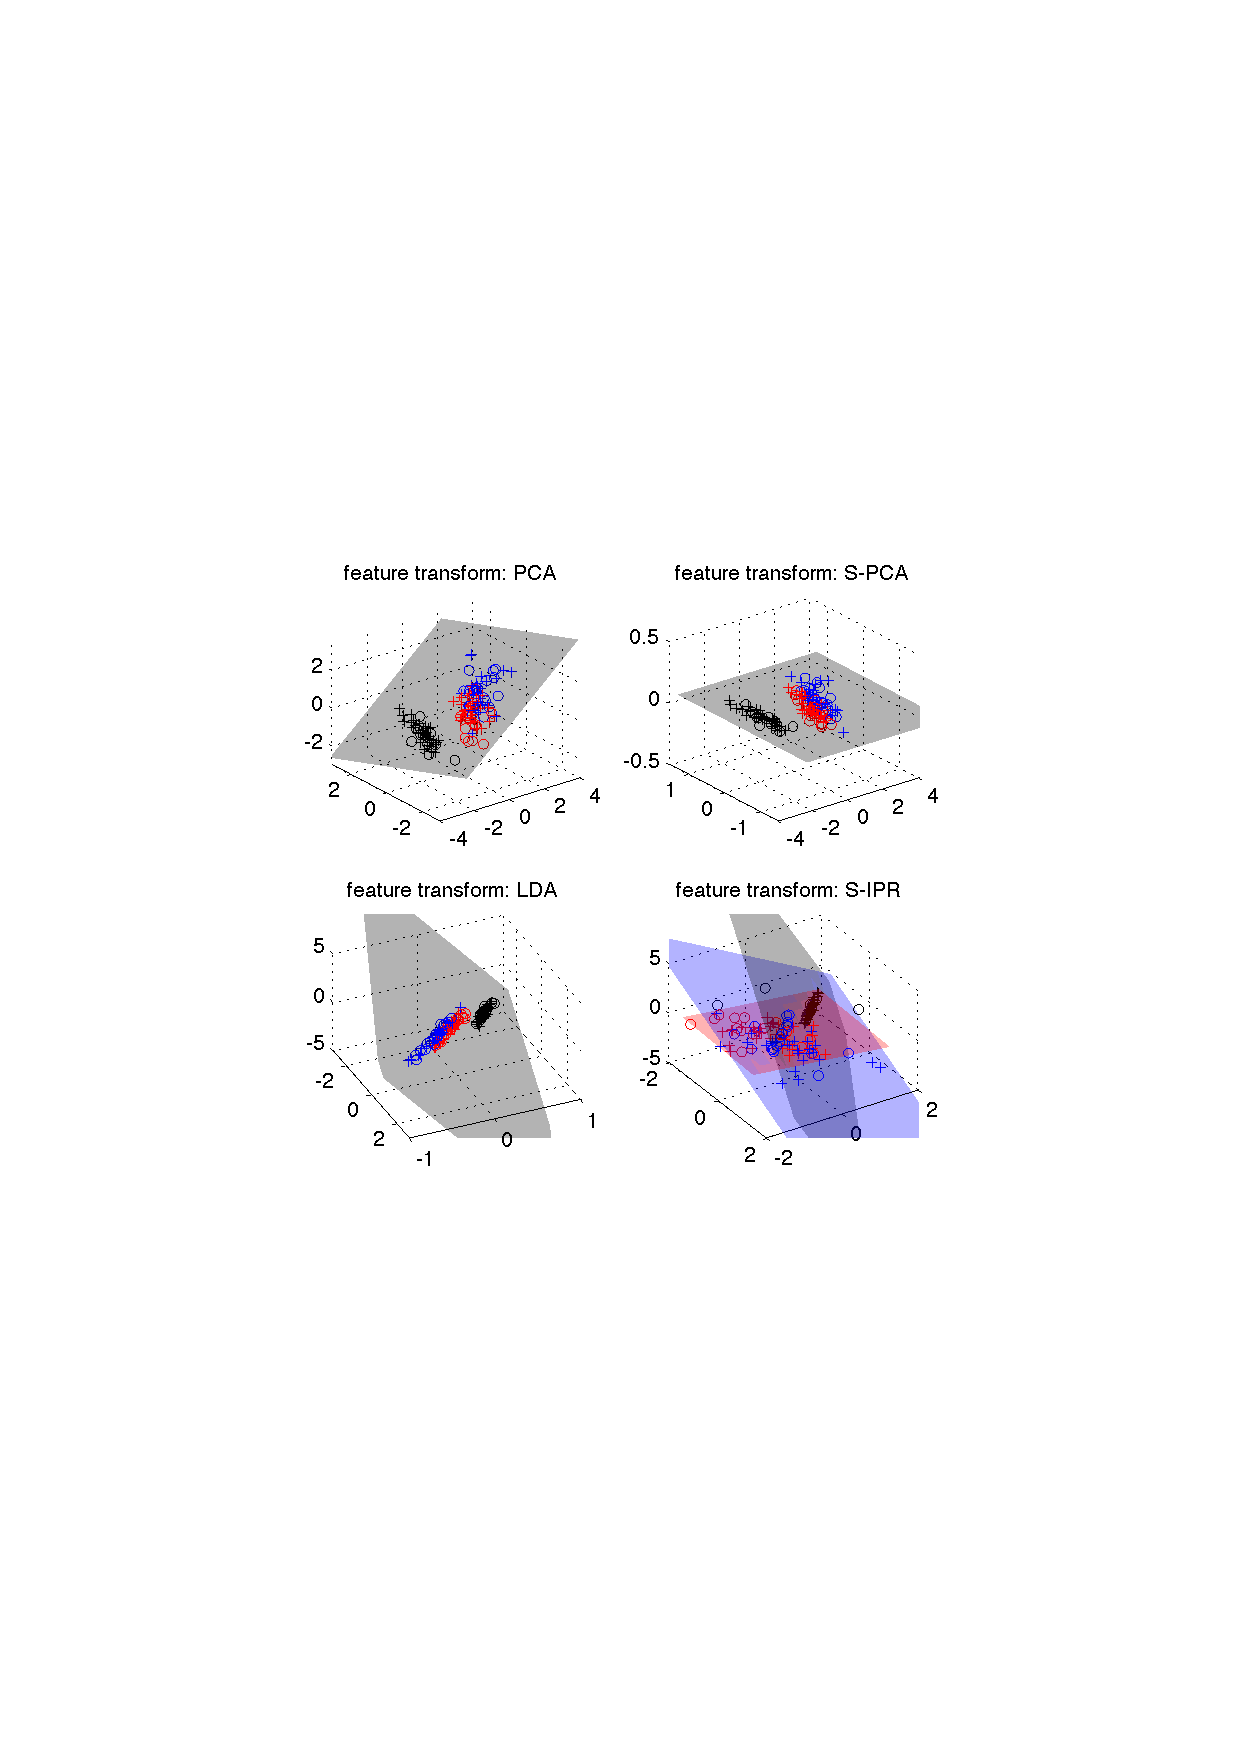
\includegraphics[width=\textwidth]{./Code/fishervisu.pdf}
\caption{\label{fig:toy}Synthetic data generated along one-dimensional subspaces of $\real^{2}$.}
\end{figure}

\subsection{Classifying the \Acronym{fisheriris} dataset}\label{sec:fisher}
To illustrate the \Acronym{s-ipr} algorithm for feature transform, we apply it to the $\Acronym{fisheriris}$ dataset \cite{Fisher1936Th}. This contains data for the classification of $150$ iris specimens into the classes \emph{setosa}, \emph{versicolor} and \emph{virginica}. The features corresponding to measurements on the sepal length, sepal width and petal length for the flowers are stored in the matrix $\Feas\in\ambient^{3\times 150}$.  As a pre-processing step, we subtract the mean and normalise the standard deviation of the features to avoid large variations or offsets in any of the dimensions of the data.

The dictionary learning is run using the \Acronym{SMALLBox} toolbox and the Incoherent dictionary learning add-on\footnote{http://code.soundsoftware.ac.uk/projects/smallbox.}. We learn an over-complete dictionary $\Dic$ consisting of $\nAto=10$ atoms and a sparse approximation $\Coeff$ that uses $\nActiveAtoms=2$ active atoms for each signal. Incoherent sub-dictionaries are learned by the \Acronym{s-ipr} method, setting the mutual coherence to the theoretical lower bound attainable by a $\nDim\times \nAto$ dictionary $\mu_{\Label{min}} = \sqrt{(\nAto-\nDim)/\nDim(\nAto-1)}\approx 0.5$ \cite{Strohmer2003Gr}. A maximum number of $\nIter=20$ iterations is set as the stopping criterion. These parameters are within the range used in previous studies of incoherent dictionary learning \cite{Barchiesi2013Le}, and have not been optimised for this task.

The proposed method is used to learn $\nDimSub=1$ dimensional sub-spaces, and is  compared to \Acronym{pca} with a number of components $\nComponents=2$ and to \Acronym{lda}. Figure \ref{fig:fisher} shows the results of the experiment. The original features show a clear cluster corresponding to the setosa class, and overlapping data for the other two classes. Applying \Acronym{pca} reduces the dimensionality of the $3$-dimensional features to a rank $2$ principal sub-space, but worsens the separation between classes. Both \Acronym{lda} and the proposed method are able to improve the separation of the three classes, but in remarkably different ways: while the former optimises the linear separability of different classes, features derived from \Acronym{s-ipr} are projected onto low-dimensional discriminative subspaces.

To assess the classification performance of the various techniques, we created a random $5$-fold partition of the training set used for cross-validation, and classified the transformed features using \Acronym{knn} with $5$ neighbours. The misclassification rate $\Acronym{mcr}$ defined as the number of misclassified samples divided by the total number of samples is displayed for the various methods in the first row of Table \ref{tab:fisher}. \Acronym{s-ipr} and \Acronym{lda} are both able to attain a $7\%$ misclassification error, improving on the $10\%$ obtained on the original features. The worst result is achieved by \Acronym{pca}, whose dimensionality reduction has the effect of mixing together features belonging to different classes, and achieves an error of $44\%$.
\begin{figure*}[!tb]
\begin{center}
%\includegraphics[width=\textwidth]{fisher3d.pdf}
\caption{\label{fig:fisher}Features transform for the fisheriris dataset. Red circular markers correspond to setosa, green square markers to versicolor and blue diamond markers to virginica.}
\end{center}
\end{figure*}
\begin{table}[!htb]
\begin{center}
\begin{tabular}{|l|c|c|c|c|}
\hline
  & none & \Acronym{pca} & \Acronym{lda} & \Acronym{s-ipr} \\
  \hline
  \textbf{\Acronym{mcr} - \Acronym{fisheriris}} & 0.10 & 0.44 & 0.07 & 0.07\\
\textbf{\Acronym{mcr} - \Acronym{usps}} & 0.343 & 0.433 & 0.359 & 0.315 \\
\hline
\end{tabular}
\caption{\label{tab:fisher} Misclassification error evaluated using different feature transform methods on the \Acronym{fisheriris} and \Acronym{usps} datasets (none indicates no feature transform).}
\end{center}
\end{table}
\subsection{Classification of the \Acronym{usps} digits dataset}
In order to evaluate the proposed method on a more challenging dataset that  contains signals of higher dimension, we run a similar experiment on the \Acronym{usps} digits dataset, which consists of a collection of $16\times 16$ pixels images of hand-written digits \footnote{http://www.cs.nyu.edu/~roweis/data.html.}. We selected the digits \Acronym{1}, \Acronym{3} and \Acronym{8} resulting in a total of $1405$ examples stored in the matrix $\Feas\in\ambient^{256\times 1405}$.

We investigated the effect of the parameters \\ $\nAto=\curlyb{256,512,1024}$, $\nDimSub=\curlyb{2,4,8,16,32,64,128}$ and $\nActiveAtoms = \curlyb{2,25,128,256}$ on the misclassification error, and compared the \Acronym{s-ipr} to \Acronym{pca} and \Acronym{lda}. For \Acronym{pca}, the number of principal components $\nComponents$ is automatically set by the algorithm to choose an approximation that retains $95\%$ of the variance of the data. The second row of Table \ref{tab:fisher} shows the results obtained with the best choice of parameters $\optimal{\nAto}=512$ (corresponding to a 2 times over-complete dictionary), $\optimal{\nDimSub}=64$ and $\optimal{\nActiveAtoms}=128$. In this case, \Acronym{s-ipr} achieves a $31.5\%$ misclassification error, while the other two techniques do not improve the \Acronym{k-nn} classification on to the original features, which scores $34.3\%$. 

Analysing the \Acronym{mcr} as a function of the parameters $\nAto$, $\nDimSub$ and $\nActiveAtoms$, the most relevant trend observed empirically on this dataset is that a value $\nDimSub<16$ steeply increases the misclassification error. This suggests that the dimensionality of the incoherent sub-spaces must be large enough to retain discriminative characteristics of the original high-dimensional data. The dependency of \Acronym{mcr} on the other two parameters is less significant, suggesting that dictionary learning leads to discriminative subspaces regardless of the number of active atoms $\nActiveAtoms$ or the number of atoms in the dictionary $\nAto$. 
\section{Conclusion}\label{sec:end}
We have presented the \Acronym{s-ipr} algorithm for learning incoherent subspaces, and employed it as a feature transform method in the context of supervised classification. The encouraging experimental results obtained on the \Acronym{fisheriris} and the \Acronym{usps} datasets suggest that the proposed algorithm can overcome limitations of standard feature transforms methods, making it a viable tool for machine learning research and practice. A better theoretical understanding of the performance of \Acronym{s-ipr} (especially in relation to other methods for subspace and manifold learning), and further validations of the technique on challenging classification problems constitute the most promising avenues for future research.

% References should be produced using the bibtex program from suitable
% BiBTeX files (here: strings, refs, manuals). The IEEEbib.bst bibliography
% style file from IEEE produces unsorted bibliography list.
% -------------------------------------------------------------------------
\bibliographystyle{IEEEbib}
\bibliography{bibliography.bib}

\end{document}
